\documentclass[research]{fcs}

\usepackage{subcaption}
\usepackage{xspace}
\usepackage{tabularx}

\makeatletter
\@ifclassloaded{fcs}{}{\AtBeginDocument{\maketitle}}
\makeatother

\graphicspath{{figures/}}
\newcommand{\method}{VulTriage\xspace}
\newcommand{\av}{\alpha_{\mathrm{v}}}
\newcommand{\as}{\alpha_{\mathrm{s}}}

\title{VulTriage: Detector-Conditional Support for Auditable Cross-Project Vulnerability Triage}
\shorttitle{VulTriage: Detector-Conditional Support for Vulnerability Triage}
\author[1,+]{Yanbo~Bian}
\author[2,+]{Zhihai~Wang}
\address[1]{Computer Science and Technology Program, Weihai International College, Beijing Jiaotong University, Weihai 264401, China}
\address[2]{School of Computer Science and Technology, Beijing Jiaotong University, Beijing 100044, China}
\corremail{24722081@bjtu.edu.cn; zhhwang@bjtu.edu.cn}
\fcssetup{
  received = {month dd, yyyy},
  accepted = {month dd, yyyy},
  article-id = {1},
  first-page = {1},
}

\begin{abstract}
Cross-project vulnerability detectors must decide when an automatic label is defensible, not only rank functions. We present \method, a post-hoc triage layer that combines class-asymmetric weighted conformal sets with a frozen, label-free support gate. The gate returns a singleton decision only when effective sample size, test-point mass, domain-shift, and clipping diagnostics pass; otherwise it returns a review set. We preregistered a sealed evaluation on 24 project groups from the public PrimeVul development release and 24 external DiverseVul projects, using a hashing-SGD detector and a frozen CodeBERT encoder with a liblinear head, five seed addresses, a 3 $\times$ 3 risk-budget grid, and 25 recorded methods. At $(\av,\as)=(0.10,0.20)$, estimated weighting reduced hashing-SGD's project-paired maximum relative budget violation by 0.816 (95\% project-bootstrap confidence interval [0.318, 1.722] for the reduction; 24/24 projects improved) while reducing singleton coverage by 15.9 percentage points. The same weighting produced no overall risk improvement for CodeBERT. The support gate had poor PrimeVul leave-one-project-out development discrimination (AUROC 0.35), but discriminated severe raw violations on external DiverseVul for hashing-SGD (AUROC 0.86) and not for CodeBERT (AUROC 0.43). Calibration-size and near-duplicate sensitivities preserved the detector-conditional pattern. These results support auditable partial automation for a lightweight detector, with an explicit review cost; they do not provide a target-risk guarantee or detector-general support certificate.
\end{abstract}

\keywords{Vulnerability detection; Cross-project shift; Conformal prediction; Selective prediction; Support diagnostics; Software security}

\begin{document}

\section{Introduction}

A vulnerability detector deployed on an unseen software project must answer two different questions. The first is predictive: which functions look vulnerable? The second is operational: which of those decisions can be automated under an asymmetric error budget? A missed vulnerable function and an unnecessary alert consume different security resources. A high confidence score by itself does not reveal whether the calibration evidence remains relevant to the new project, nor whether a desired vulnerable-class risk budget is supported by enough effective observations.

Public vulnerability benchmarks have made the first question more realistic. PrimeVul reports the effects of duplicate functions, label quality, imbalance, and evaluation design on code-language-model results \cite{ding2025primevul}, while DiverseVul broadens project and weakness coverage for deep vulnerability detection \cite{chen2023diversevul}. Cross-project methods address representation and distribution mismatch with transfer learning, domain adaptation, graph representations, and zero-shot mechanisms \cite{lin2018transfer,liu2022cdvuld,zhang2023cpvd,nguyen2024dam2p,cai2024csvdtf,haque2026zsvuld}. These methods improve or adapt a detector, but a deployment still needs an explicit policy for returning a label, deferring to review, and reporting the cost of that refusal.

Calibration and selective prediction provide useful ingredients. CodeBERT is a standard pretrained representation for source code \cite{feng2020codebert}, and LineVul and data-flow-aware models show how detector architecture can be improved \cite{fu2022linevul,steenhoek2024deepdfa}. Temperature scaling is a canonical calibration baseline \cite{guo2017calibration}, while selective prediction formalizes the risk--coverage trade-off \cite{geifman2019selectivenet}. Code-model calibration can degrade under shift \cite{zhou2024calibration}, and Prom provides a deployment-time conformal assessment for code-analysis tasks \cite{wang2025prom}. Recent work also frames code prediction as an answer-or-defer decision \cite{rathnasuriya2026defer}. None of these observations, however, makes a class-asymmetric support decision for cross-project vulnerability triage a validated deployment interface.

We study \method, a detector-agnostic post-hoc layer with an explicitly detector-conditional evaluation. It constructs class-conditional prediction sets using estimated source-to-target relevance weights, then applies a frozen support gate based only on unlabeled target code and source calibration diagnostics. A singleton set is an automatic label; a doubleton is review. The gate is not treated as a risk certificate. Instead, we test whether its label-free pass signal predicts severe raw violation after labels are released, separately for each detector.

The study asks:

\begin{itemize}
  \item \textbf{RQ1:} Does support qualification yield nontrivial, auditable automation on unseen projects?
  \item \textbf{RQ2:} Does estimated target weighting align class-asymmetric sets with requested risk budgets, and is the result detector-independent?
  \item \textbf{RQ3:} What are the costs and validity boundaries of refusal, calibration size, duplicate control, and computation?
\end{itemize}

The contributions are fourfold:

\begin{enumerate}
  \item a preregistered, prediction-sealed benchmark that combines a PrimeVul development domain, a DiverseVul external domain, two detectors, five frozen seed addresses, a 3 $\times$ 3 asymmetric risk grid, and 25 methods;
  \item a positive but bounded result: on hashing-SGD, target weighting decreases the worst relative budget violation on all 24 projects at the primary operating point, with a quantified 15.9 percentage-point singleton-coverage cost;
  \item an external validity test showing that the frozen gate discriminates severe raw violation for hashing-SGD but not for CodeBERT, while retaining the negative PrimeVul development AUROC of 0.35; and
  \item released summaries, sensitivity analyses, figure source data, efficiency observations, validation manifests, and a public builder that excludes raw code, labels, embeddings, private indexes, and per-function decision archives.
\end{enumerate}

\section{Related work}

\subsection{Cross-project vulnerability detection}

Representation transfer for vulnerable-function discovery predates current code-language models \cite{lin2018transfer}. CD-VulD combines deep domain adaptation with cross-domain vulnerability discovery \cite{liu2022cdvuld}. CPVD uses graph attention and domain adaptation \cite{zhang2023cpvd}, DAM2P introduces a max-margin domain-adaptation objective for imbalanced data \cite{nguyen2024dam2p}, and CSVD-TF uses TrAdaBoost to fuse expert and semantic metrics \cite{cai2024csvdtf}. ZSVulD studies a zero-shot setting with pretrained representations and collaborative classifiers \cite{haque2026zsvuld}. These systems change the detector or its training objective. \method is complementary: it takes a fitted detector and exposes a decision layer that can refuse unsupported automation.

Modern code detectors provide important external-validity baselines. CodeBERT supplies a pretrained code representation \cite{feng2020codebert}, LineVul adapts transformers to line-level vulnerability prediction \cite{fu2022linevul}, and DeepDFA injects data-flow structure for efficient detection \cite{steenhoek2024deepdfa}. Our CodeBERT track is deliberately a frozen encoder plus a source-train-only standardized logistic head, not a claim of fine-tuned state of the art. The contrast with hashing-SGD therefore tests whether support-aware weighting behaves consistently across a low-cost lexical detector and a semantic representation.

\subsection{Calibration, deferral, and conformal risk}

Temperature scaling changes probability calibration but not the binary ranking \cite{guo2017calibration}. Selective prediction makes retained coverage an explicit companion to risk \cite{geifman2019selectivenet}, and code-model studies show that calibration remedies can behave differently under project or temporal shift \cite{zhou2024calibration,li2021shift}. Prom uses local conformal experts, including LAC, TopK, APS, and RAPS, to identify deployment-time errors in code analysis \cite{wang2025prom}. We use a preregistered binary, deterministic PROM-derived adapter as a strong comparison, while distinguishing it from the official implementation. The answer-or-defer perspective for code prediction is also established \cite{rathnasuriya2026defer}; our focus is the security-specific separation of vulnerable and safe budgets and the validity of an unlabeled support signal.

Weighted conformal prediction can recover target marginal coverage under covariate shift when the likelihood ratio is known and conditional labels are invariant \cite{tibshirani2019weightedcp}. Conformal risk control generalizes the controlled loss \cite{angelopoulos2024crc}, and nonexchangeable or high-probability variants make the shift assumptions explicit \cite{farinhas2024necrc,almeida2025hpcrc}. Our density ratios are learned from a finite domain classifier and project shift may include concept shift. We therefore report empirical violation, support diagnostics, and refusal cost rather than claiming a distribution-free deployment guarantee.

\section{VulTriage}

\subsection{Three-way action interface}

Let $Y\in\{0,1\}$ denote safe and vulnerable, respectively, and let a fitted detector output class probabilities $\widehat p_y(x)$. For calibration example $(x_i,y_i)$, the label-conditional nonconformity score is

\begin{equation}
 S_i=1-\widehat p_{y_i}(x_i).
\end{equation}

The output $\Gamma(x)\subseteq\{0,1\}$ has three operational interpretations. $\{0\}$ and $\{1\}$ are singleton automatic decisions; $\{0,1\}$ is a review decision. Empty sets, which can arise in comparison methods, are also routed to review and are recorded separately. For class $y$, the empirical miscoverage is

\begin{equation}
 R_y=\Pr\{y\notin\Gamma(X)\mid Y=y\}.
\end{equation}

The user supplies $\alpha_1=\av$ and $\alpha_0=\as$. Singleton coverage is $\Pr(|\Gamma(X)|=1)$ and review load is its complement.

\subsection{Asymmetric weighted sets}

For class $y$, let $\mathcal I_y$ be its calibration indices and let $w_i$ be estimated target relevance weights. For a target point with weight $w(x)$, the implemented threshold is

\begin{equation}
q_y(x)=\inf\left\{t:\sum_{i\in\mathcal I_y} w_i\mathbf 1(S_i\leq t)\geq(1-\alpha_y)\left(\sum_{i\in\mathcal I_y}w_i+w(x)\right)\right\}.
\label{eq:weighted}
\end{equation}

If the calibration mass cannot reach the right-hand side, $q_y(x)=\infty$. The set contains class $y$ when $1-\widehat p_y(x)\leq q_y(x)$. Unit weights recover unweighted Mondrian conformal prediction. The weighted construction is an empirical post-processing rule: its exact covariate-shift validity would require a correct likelihood ratio and invariant conditional labels \cite{tibshirani2019weightedcp}.

\subsection{Project-shift weights and support gate}

For each held-out project, a source--target domain classifier is trained with five deterministic cross-fitting folds. Equal source and target sampling makes the cross-fitted target odds

\begin{equation}
 \widehat w(x)=\frac{\widehat P(D=1\mid x)}{1-\widehat P(D=1\mid x)}
\end{equation}

an estimated relevance ratio. The primary weights are clipped to $[1/20,20]$; clips 10 and 50 are sensitivity variants. The same label-free weights are shared by detector-head seeds.

The frozen support gate is fitted only on 12 PrimeVul project-disjoint pseudo-targets using leave-one-project-out cross-fitting. Its features are log total and class-specific Kish effective sample sizes (ESS), maximum and 99th-percentile test-point infinity mass, domain-classifier AUROC, and lower and upper clipping fractions. The gate predicts whether the raw weighted policy will have severe relative violation, defined as

\begin{equation}
 \max\left(\frac{\max(0,R_1-\av)}{\av},\frac{\max(0,R_0-\as)}{\as}\right)>0.5.
\end{equation}

The final gate passes only when its predicted severe-violation probability is below 0.5 and at least one singleton exists. Missing or nonfinite diagnostics fail closed. A failed gate replaces the entire target-project cell with review sets. This is a conservative refusal policy, not evidence that the requested risks have been attained.

\begin{figure*}[t]
  \centering
  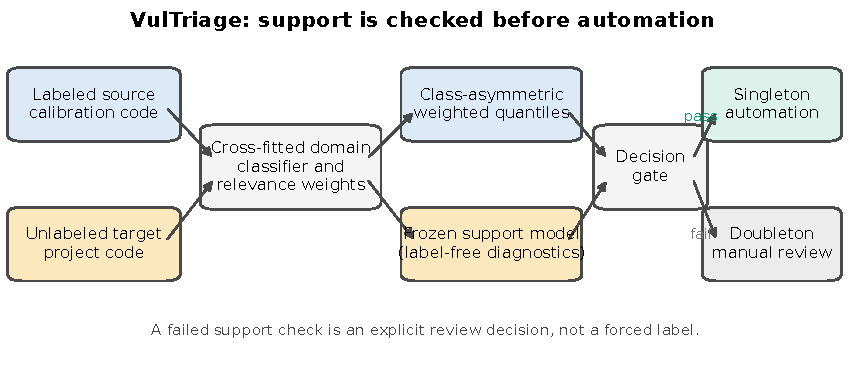
\includegraphics[width=0.96\textwidth]{fig1_workflow.pdf}
  \caption{\method uses labeled source calibration code and unlabeled target-project code to estimate relevance, construct class-asymmetric weighted sets, and apply a frozen support model before automation. A failed support check returns a review set rather than a forced label.}
  \label{fig:workflow}
\end{figure*}

\section{Frozen study design}

\subsection{Datasets and project splits}

The development domain is the original public PrimeVul release \cite{ding2025primevul}. After deterministic canonicalization and exact deduplication, the source package contains 226,582 functions from 235,768 valid rows; 9,186 same-label duplicates are removed and no conflicting label keys are retained. For each external target, source rows are partitioned by salted commit-hash buckets into 70\% detector training, 10\% model validation, and 20\% calibration. Project aliases are frozen before model output.

The external confirmation domain is the official public DiverseVul release \cite{chen2023diversevul}. We select 24 eligible project groups without inspecting model outcomes, require at least 200 total, 20 vulnerable, and 20 safe functions, and then exact-deduplicate across datasets. The resulting target cohort contains 79,355 functions. Labels remain in a separate vault until both detector prediction seals are verified. The primary cohort is unchanged by the near-duplicate sensitivity analysis.

\begin{table*}[t]
\centering
\caption{Frozen DiverseVul external project groups. Target rows are exact-deduplicated functions; vulnerability prevalence is reported only descriptively after label release.}
\label{tab:projects}
\small
\begin{tabular}{lrrr@{\qquad}lrrr}
\toprule
Project & Total & Vulnerable & Prev. (\%) & Project & Total & Vulnerable & Prev. (\%)\\
\midrule
linux & 32,930 & 3,032 & 9.21 & openssl & 4,352 & 565 & 12.98\\
tensorflow & 2,677 & 438 & 16.36 & php & 3,592 & 353 & 9.83\\
qemu & 2,634 & 338 & 12.83 & imagemagick & 783 & 300 & 38.31\\
qpdf & 1,786 & 272 & 15.23 & envoy & 5,252 & 254 & 4.84\\
tcpdump & 428 & 209 & 48.83 & jasper & 608 & 203 & 33.39\\
radare2 & 1,610 & 168 & 10.43 & postgres & 2,605 & 154 & 5.91\\
mysql-server & 3,838 & 142 & 3.70 & FreeRDP & 980 & 141 & 14.39\\
libxml2 & 2,060 & 136 & 6.60 & krb5 & 491 & 118 & 24.03\\
samba & 1,961 & 117 & 5.97 & vim & 3,056 & 116 & 3.80\\
net & 1,810 & 116 & 6.41 & ffmpeg & 983 & 115 & 11.70\\
mongo & 2,627 & 112 & 4.26 & ghostpdl & 1,132 & 109 & 9.63\\
libtpms & 490 & 109 & 22.24 & librsvg & 670 & 95 & 14.18\\
\bottomrule
\end{tabular}
\end{table*}

\subsection{Detectors and comparison methods}

The lightweight detector hashes case-sensitive word unigrams and bigrams into $2^{18}$ dimensions, applies $\ell_2$ normalization, and fits a class-balanced averaged-SGD logistic head for three epochs. Regularization is selected by source-validation PR-AUC. Seeds 13, 37, 73, 101, and 137 are five independently fitted technical seeds per project.

The semantic track uses \texttt{microsoft/codebert-base} at immutable revision \texttt{3b0952feddeffad0063f274080e3c23d75e7eb39}. Final hidden states are attention-mask mean pooled after removing special tokens. A source-train-only StandardScaler feeds a class-weighted L2 liblinear logistic head; $C\in\{0.01,0.1,1,10\}$ is selected on source validation. CodeBERT is fitted once at seed 13 per project and the deterministic head is copied to the other four frozen seed addresses. This is a reproducibility address scheme, not five independent CodeBERT fits.

The evaluation records forced argmax, matched maximum-softmax and entropy, temperature-matched confidence, pooled and unweighted conformal sets, a binary PROM-derived adapter (LAC, TopK, APS, RAPS, and their union), estimated weighting with clips 10/20/50, ESS-only and infinity-mass-only gates, the full frozen gate, and matched full-gate derivatives. The PROM comparison is explicitly a deterministic binary adapter, not an official PROM reproduction \cite{wang2025prom}.

\subsection{Outcomes, sealing, and statistics}

The frozen risk grid is $\av\in\{0.01,0.05,0.10\}$ by $\as\in\{0.05,0.10,0.20\}$. Primary outcomes are vulnerable and safe miscoverage, positive class-specific violation, maximum relative violation, singleton coverage, and review load. Detector performance includes PR-AUC, F1, Matthews correlation coefficient (MCC), Brier score, expected calibration error, area under the risk--coverage curve, and error-detection AUROC. The latter ranks forced 0.5-threshold mistakes by $1-\max_y\widehat p_y$; it is not a vulnerable-classification ROC-AUC.

Prediction files are hashed and sealed before target labels are joined. The final evaluation contains 54,000 fold--seed metric rows, 10,800 project--seed averages, 450 paired comparisons, 14,400 calibration-size rows, and 6,480 near-duplicate sensitivity rows. Five seeds are averaged within each project before inference; the independent unit is the 24-project target group. Project-bootstrap intervals use 10,000 resamples. Exact Wilcoxon tests are emitted only when at least ten nonzero paired differences remain, with Holm adjustment within each detector, budget, and outcome family.

\section{Results}

\subsection{Base detectors are comparable, not interchangeable}

Table~\ref{tab:detector} summarizes the two detector tracks at the primary operating point. CodeBERT has a modestly higher median PR-AUC, F1, and MCC, but project-bootstrap intervals for PR-AUC, F1, and MCC overlap the hashing track. Its error-detection AUROC is higher, whereas its Brier score is also higher (worse). The decision-layer results below should therefore be interpreted as detector-conditional rather than as a model-superiority claim.

\begin{table}[t]
\centering
\caption{Base detector performance across 24 external projects. Values are project medians with the interquartile range in parentheses; confidence intervals are 10,000-project bootstrap intervals. Error-detection AUROC is not vulnerable-class ROC-AUC.}
\label{tab:detector}
\small
\begin{tabular}{lcc}
\toprule
Metric & Hashing-SGD & CodeBERT\\
\midrule
PR-AUC & 0.188 (0.149--0.295) & 0.193 (0.141--0.278)\\
F1 & 0.268 (0.197--0.343) & 0.271 (0.186--0.366)\\
MCC & 0.162 (0.113--0.198) & 0.183 (0.143--0.233)\\
Brier (lower) & 0.194 (0.151--0.240) & 0.203 (0.173--0.236)\\
Error-detection AUROC & 0.677 (0.625--0.733) & 0.718 (0.654--0.762)\\
\bottomrule
\end{tabular}
\end{table}

\subsection{Support is detector-conditional}

Figure~\ref{fig:gate} combines the negative development result with the external confirmation. The frozen gate has PrimeVul leave-one-project-out AUROC 0.35 and AUPRC 0.2452 over 108 development cells. On DiverseVul, it has AUROC 0.8601 and AUPRC 0.8173 for hashing-SGD; pass projects have a median raw maximum-relative-violation difference of $-0.5473$ versus fail projects (95\% interval $[-1.0057,-0.2244]$). For CodeBERT the AUROC is 0.4286. Its AUPRC 0.8733 is close to the severe-event prevalence of 0.875, and the pass--fail interval $[-2.4498,0.7270]$ crosses zero. The gate therefore has external discrimination for hashing-SGD, not a detector-general support signal.

\begin{figure*}[t]
  \centering
  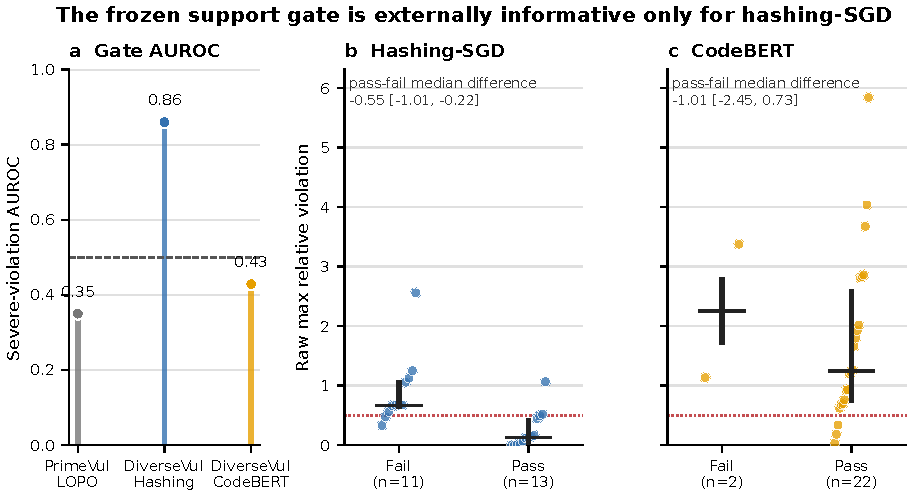
\includegraphics[width=0.96\textwidth]{fig2_gate_validity.pdf}
  \caption{Detector-conditional validity of the frozen support gate. (a) Severe-violation AUROC includes the negative PrimeVul development result and the two DiverseVul external detector tracks; the dashed line is chance. (b,c) Raw maximum-relative violation by all-five-seed gate status at the primary operating point. Points are projects; black marks show the interquartile range and median; the red dotted line is the severe-violation threshold. Pass--fail differences are descriptive associations, not causal effects.}
  \label{fig:gate}
\end{figure*}

\subsection{Weighting improves risk alignment for hashing-SGD}

At $(\av,\as)=(0.10,0.20)$, estimated weighting with clip 20 reduces hashing-SGD maximum relative violation by a median 0.8161 compared with unweighted Mondrian sets (95\% project-bootstrap interval for the signed difference $[-1.7219,-0.3174]$; 24/24 project directions improve; Holm-adjusted exact Wilcoxon $p=5.96\times10^{-7}$). Vulnerable-class violation decreases by 0.0853 (23 wins, one tie; adjusted $p=1.19\times10^{-6}$). Safe-class violation has no stable change (median difference 0.0000; adjusted $p=0.9748$). The corresponding 0.1587 reduction in singleton coverage occurs in all 24 projects (adjusted $p=5.96\times10^{-7}$), so the risk alignment is not free automation.

The detector contrast is decisive. CodeBERT's maximum-relative-violation difference is $-0.0052$ with interval $[-0.2837,0.5505]$ and 12 wins versus 12 losses (adjusted $p=1$). Vulnerable violation is directionally worse by 0.0298, while safe violation improves by 0.0075; singleton-coverage change is $-0.0235$ with an interval crossing zero. Across all nine budget cells, the weighted hashing policy improves, ties, or worsens 202, 6, or 8 of 216 project--budget cells; CodeBERT gives 97, 32, or 87. These cell counts are descriptive because the nine cells within a project are correlated.

\begin{figure*}[t]
  \centering
  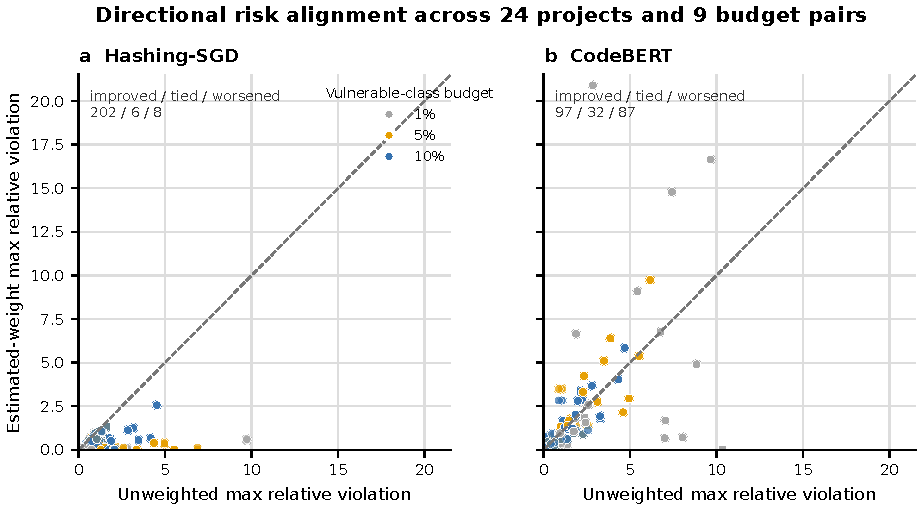
\includegraphics[width=0.94\textwidth]{fig4_risk_alignment.pdf}
  \caption{Directional risk alignment over the 24 projects and nine frozen budget pairs. Each point compares raw estimated-weight sets with unweighted Mondrian sets; points below the diagonal improve maximum relative violation. Colors encode the vulnerable-class budget. The improved/tied/worsened counts are descriptive cell counts, not independent sample sizes.}
  \label{fig:alignment}
\end{figure*}

\subsection{Automation is measurable, but gate failure can create mechanical attainment}

At the primary operating point, the full gate supports 13/24 hashing projects and 22/24 CodeBERT projects. Among supported hashing projects, median singleton coverage is 0.509 and maximum relative violation is 0.122; only 2/13 supported projects attain both class budgets after labels are released. For CodeBERT, supported median coverage is 0.749, maximum relative violation is 1.244, and supported attainment is 0/22. The apparent overall full-gate attainment of 13/24 for hashing and 2/24 for CodeBERT is therefore dominated by gate-fail projects that are sent entirely to review and consequently have zero automatic violation. We do not count those mechanical zeros as evidence of predictive risk control.

Figure~\ref{fig:automation} shows the corresponding supported-project coverage. The hashing median is 50.9\% and the CodeBERT median is 74.9\%. The difference is operationally important: a system that refuses more often can look safer while increasing analyst workload. PROM-derived APS and RAPS provide another reminder of this trade-off, with about 24--26\% coverage and higher descriptive attainment; TopK and the PROM union reject every function. These baselines are retained as controls, not presented as practical dominance.

\begin{figure*}[t]
  \centering
  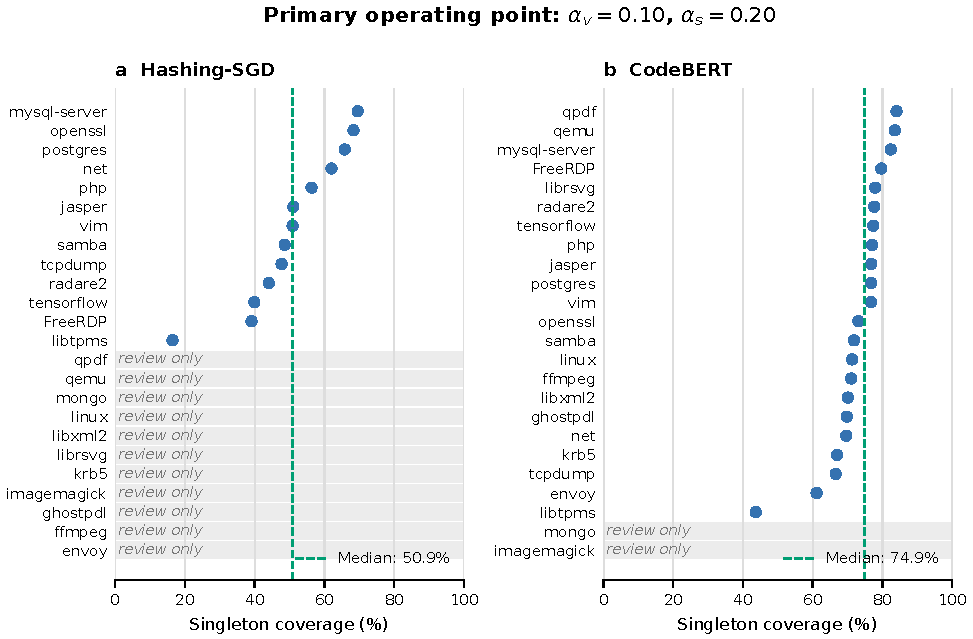
\includegraphics[width=0.94\textwidth]{fig3_primary_automation.pdf}
  \caption{Singleton coverage at $(\av,\as)=(0.10,0.20)$. Each point is a supported project; gray rows are gate-fail projects routed entirely to review. The dashed line is the median coverage among supported projects. Coverage is not target-risk attainment.}
  \label{fig:automation}
\end{figure*}

\subsection{Sensitivity and resource observations}

The calibration-size sensitivity preserves the central detector contrast (Fig.~\ref{fig:calibration}). For hashing-SGD, weighted versus unweighted median maximum relative violation is 0.099 versus 1.271 at 25\% calibration, and 0.483 versus 1.242 at 100\%; weighted coverage rises from 35.5\% to 52.4\% while remaining below unweighted coverage of 69.4\% to 69.7\%. Full-gate pass rates rise from 0 at 25\% to 0.542 at 100\%, but the 25\% full-gate zero attainment is entirely review-only. CodeBERT has no consistent weighting advantage: its weighted maximum relative violation is 1.290, 1.296, 1.295, and 1.244 across the four fractions, versus 1.270, 1.224, 1.219, and 1.238 unweighted.

The near-duplicate audit generated 866,094 approximate-LSH candidates and exactly verified every candidate. It flagged 24,606 pairs at lexical-token Jaccard at least 0.90, affecting 15,026 of 79,355 target rows (18.94\%) and retaining 64,329 rows. Recomputing sealed decisions on the clean sensitivity cohort preserves the hashing direction: weighted maximum relative violation changes from 0.483 to 0.434 and coverage from 0.524 to 0.528, whereas CodeBERT changes from 1.244 to 1.799 and from 0.749 to 0.769. This is a sensitivity re-evaluation, not a refit.

\begin{figure*}[t]
  \centering
  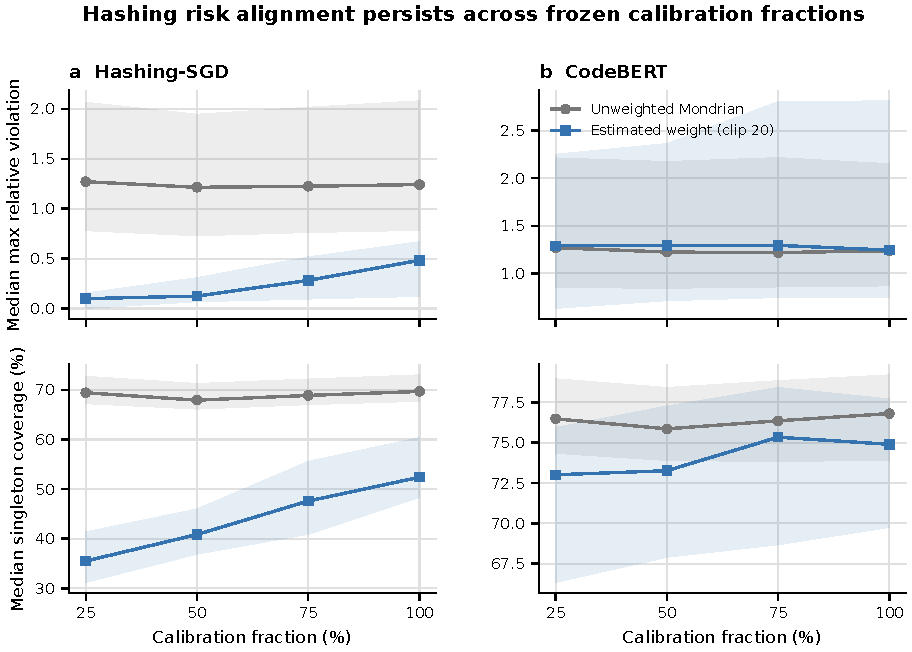
\includegraphics[width=0.94\textwidth]{fig5_calibration_sensitivity.pdf}
  \caption{Calibration-size sensitivity at the primary budget. Lines show project medians and ribbons show the interquartile range across 24 projects. Weighted hashing retains lower maximum relative violation at every fraction but lower singleton coverage; CodeBERT has no consistent risk-alignment advantage.}
  \label{fig:calibration}
\end{figure*}

The efficiency audit is observational. Hashing executes 120 independent head fits with a median 1.83 s fit duration, whereas CodeBERT executes 24 actual deterministic head fits with a median 1,584 s duration after 1,522 s of embedding extraction. CodeBERT runs in four concurrent parts; hashing is recorded as a sequential pipeline. Because hardware, batching, and parallelization differ, these numbers do not support a speedup, energy, or architecture-efficiency claim. They do support reporting the resource cost of the semantic track and the seed-reuse policy.

\section{Discussion}

\subsection{What the positive result supports}

The strongest conclusion is a decision-layer result for a lightweight detector. When relevance weighting is applied without the gate, the hashing track reduces class-asymmetric risk exceedance across projects and budget cells. The effect survives a smaller calibration cohort and a restrictive near-duplicate sensitivity cohort. A deployer can therefore use the method as an auditable risk--coverage surface: choose budgets, inspect label-free support, and decide how much review capacity is acceptable.

This result is deliberately narrower than model superiority. CodeBERT has similar base detection metrics and higher error-detection AUROC, yet the same weighting rule does not improve overall risk alignment. A support model trained on PrimeVul also performs poorly in leave-one-project-out development evaluation. The external hashing result is encouraging because it is obtained on a separate dataset, but the detector contrast means that support is a property of the detector--shift pair, not a universal certificate.

\subsection{Why support, coverage, and attainment must be separated}

Support qualification is a pre-label diagnostic. Singleton coverage measures how much automation remains after the policy. Attainment measures whether the observed target violations satisfy both budgets after labels are released. These quantities can move in opposite directions. In particular, a failed gate sends all functions to review, producing zero automatic violation and zero coverage. Reporting only overall attainment would reward refusal and conceal the operational cost. Our tables and evidence package report the supported cohort separately and keep the negative development gate result visible.

\subsection{Limitations and threats to validity}

\textbf{Construct validity.} Singleton coverage is a proxy for automation volume, not analyst time saved. We conduct no human productivity study. A safe singleton is not a security certification, and empirical budget attainment is not a finite-sample guarantee.

\textbf{Internal validity.} Prediction seals prevent target-label access during model output, and exact deduplication plus alias maps are frozen. Public benchmark labels can still be incomplete or noisy. CodeBERT seed addresses are deterministic copies of one head per project, so they do not quantify independent encoder or optimization variation. The gate pass--fail comparison is associational, not causal.

\textbf{Statistical conclusion validity.} The independent sample is 24 projects, not 120 seed--project cells or 216 independent budget cells. Bootstrap intervals quantify project heterogeneity. Holm correction is restricted to the preregistered comparator family within each detector, budget, and outcome. Sensitivity fractions and near-duplicate rows are descriptive re-evaluations.

\textbf{External validity.} The study covers public C/C++ functions and two detector tracks. It does not establish behavior for fine-tuned CodeBERT, LineVul, data-flow models, other languages, private repositories, or concept shifts with changing vulnerability mechanisms. The positive hashing result requires replication with independently fitted semantic detectors and additional external projects.

\subsection{Data and code availability, ethics, and reproducibility}

PrimeVul and DiverseVul are public defensive-use datasets released by their respective authors \cite{ding2025primevul,chen2023diversevul}. The public repository at \url{https://github.com/bianyanbo44-afk/vultriage-fcs} contains the frozen protocol, label-free source and target metadata, evaluation and analysis code, summary tables, figure source data, efficiency summaries, evidence and validation manifests, and the manuscript build files. It excludes raw source datasets, target-label vaults, private SQLite indexes, CodeBERT embeddings, feature caches, and per-function prediction or decision archives. The extension-v2 configuration SHA-256 is \texttt{8AA39B09\allowbreak{}20D8CD2C\allowbreak{}FEFBF8C2\allowbreak{}8109754F\allowbreak{}1B2DFA60\allowbreak{}49E17565\allowbreak{}122C6968\allowbreak{}E199AAD2}; the independent artifact validation and evidence-validation reports are stored with the public snapshot.

The study uses public source-code records and vulnerability labels for defensive classification. It does not generate exploits, access live systems, or involve human participants; institutional ethics review is not applicable subject to institutional policy. The authors received no specific funding and declare no competing interests.

\subsection{Conclusion}

\method turns cross-project vulnerability uncertainty into an explicit deploy-or-review interface. In a sealed, preregistered dual-dataset study, estimated weighting improves worst-class budget alignment across all 24 DiverseVul projects for hashing-SGD at the primary operating point, with a clear 15.9 percentage-point automation cost. The result survives calibration-size and near-duplicate sensitivity, while the frozen gate shows external discrimination only for the hashing detector and not for CodeBERT. The evidence supports auditable partial automation for a lightweight detector, not universal target-risk guarantees or detector-general support validity.

\section*{Acknowledgements}
The authors received no specific funding for this work.

\section*{Competing interests}
The authors declare that they have no competing interests.

\section*{Author contributions}
Yanbo Bian: Conceptualization, Data curation, Formal analysis, Investigation, Methodology, Project administration, Software, Validation, Visualization, Writing--original draft, Writing--review and editing. Zhihai Wang: Conceptualization, Formal analysis, Methodology, Supervision, Validation, Writing--review and editing.

\bibliographystyle{fcs}
\bibliography{references}

\end{document}
